\begin{frame}
  \begin{itemize}
  \item Тег canvas (HTML5), обновляется раз в 15 секунд.
  \item starjs для расчёта положения планет, преобразования координат
    и т.п.  О.~Монтенбрук, Т.~Пфлегер. ``Астрономия на персональном
    компьютере''.
  \item Стереографическая проекция.
  \end{itemize}

  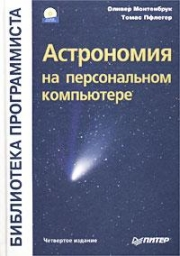
\includegraphics[widht=0.4\textwidth]{astro.jpg}

  Стереографическая проекция.  С римановой сферы на комплексную
  плоскость:
  \begin{equation}
    z = \frac{1}{z_0}
  \end{equation}
  Круги (дуги) на небесной сфере переходят в круги и прямые (дуги и
  отрезки) -- легко рисовать.  Мат. пакет Maxima для вывода формул в
  сложных случаях.
\end{frame}
%%% Local Variables: 
%%% mode: latex
%%% TeX-master: "presentation"
%%% End: 
